\chapter{Systemarkitektur}
Dette afsnit præsenterer systemets arkitektur i en grad, der gør det muligt at forstå grænsefladerne mellem hardware- og softwarekomponenter. En mere detaljeret beskrivelse for systemarkitekturen, er dokumenteret i dokumentationen afsnit 3 - \textit{Systemarkitektur}

\section{Domænemodel}
På figur \ref{figure:domainModel} ses domænemodellen for systemet. Denne har til formål at præsentere forbindelserne mellem systemets komponenter samt dets grænseflader.

\begin{figure}[H]
	\begin{adjustwidth}{-2cm}{-\rightmargin}
		\centering
		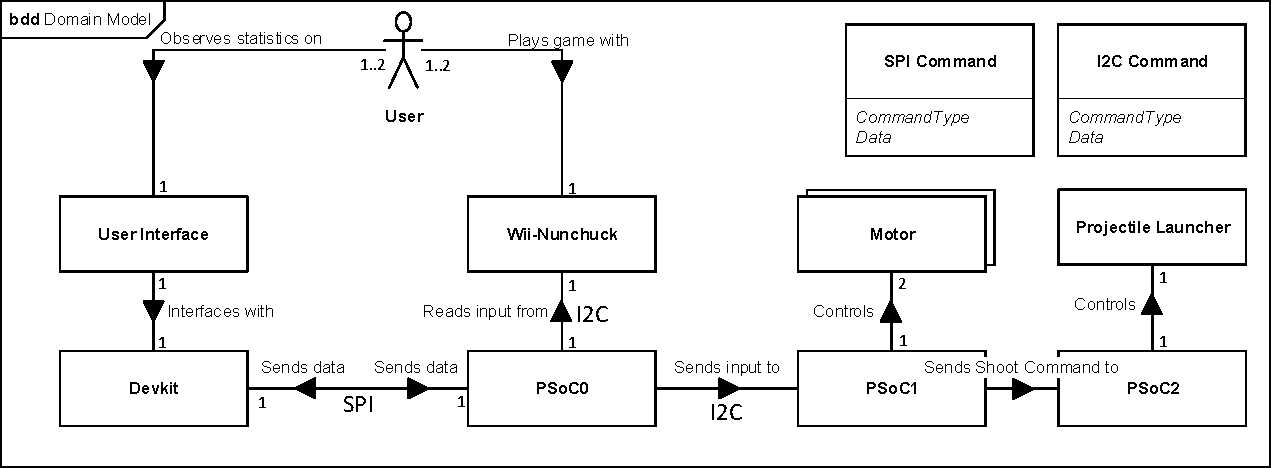
\includegraphics[width=0.75\paperwidth]{SystemArkitektur/images/domainModel}
		\caption{Systemets domænemodel}
		\label{figure:domainModel}
	\end{adjustwidth}
\end{figure}

\noindent Her repræsenteres hardware som blokke forbundet med associationer. Associationerne viser grænsefladerne mellem de forbundne hardware komponenter samt retningen af kommunikationen. Af modellen fremstår konceptuelle kommandoer for grænsefladerne, som beskriver deres nødvendige attributter. \newline

\noindent Domænemodellen er brugt til at udlede grænseflader for systemet samt potentielle hardware- og softwarekomponenter. Hvad der er udledt af domænemodellen i forhold til grænseflader og komponenter, og hvordan dette bruges, præsenteres i de følgende arkitekturafsnit. Den fulde beskrivelse af domænemodellen ses i dokumentationen afsnit 3.1-\textit{Domænemodel} side 11.

\section{Hardware}

\subsection{BDD}
\label{afsnit:BDD}
På figur \ref{figure:bddDiagram} ses BDD'et for systemet.

\begin{figure}[H]
	\begin{adjustwidth}{-3cm}{-\rightmargin}
	\centering
	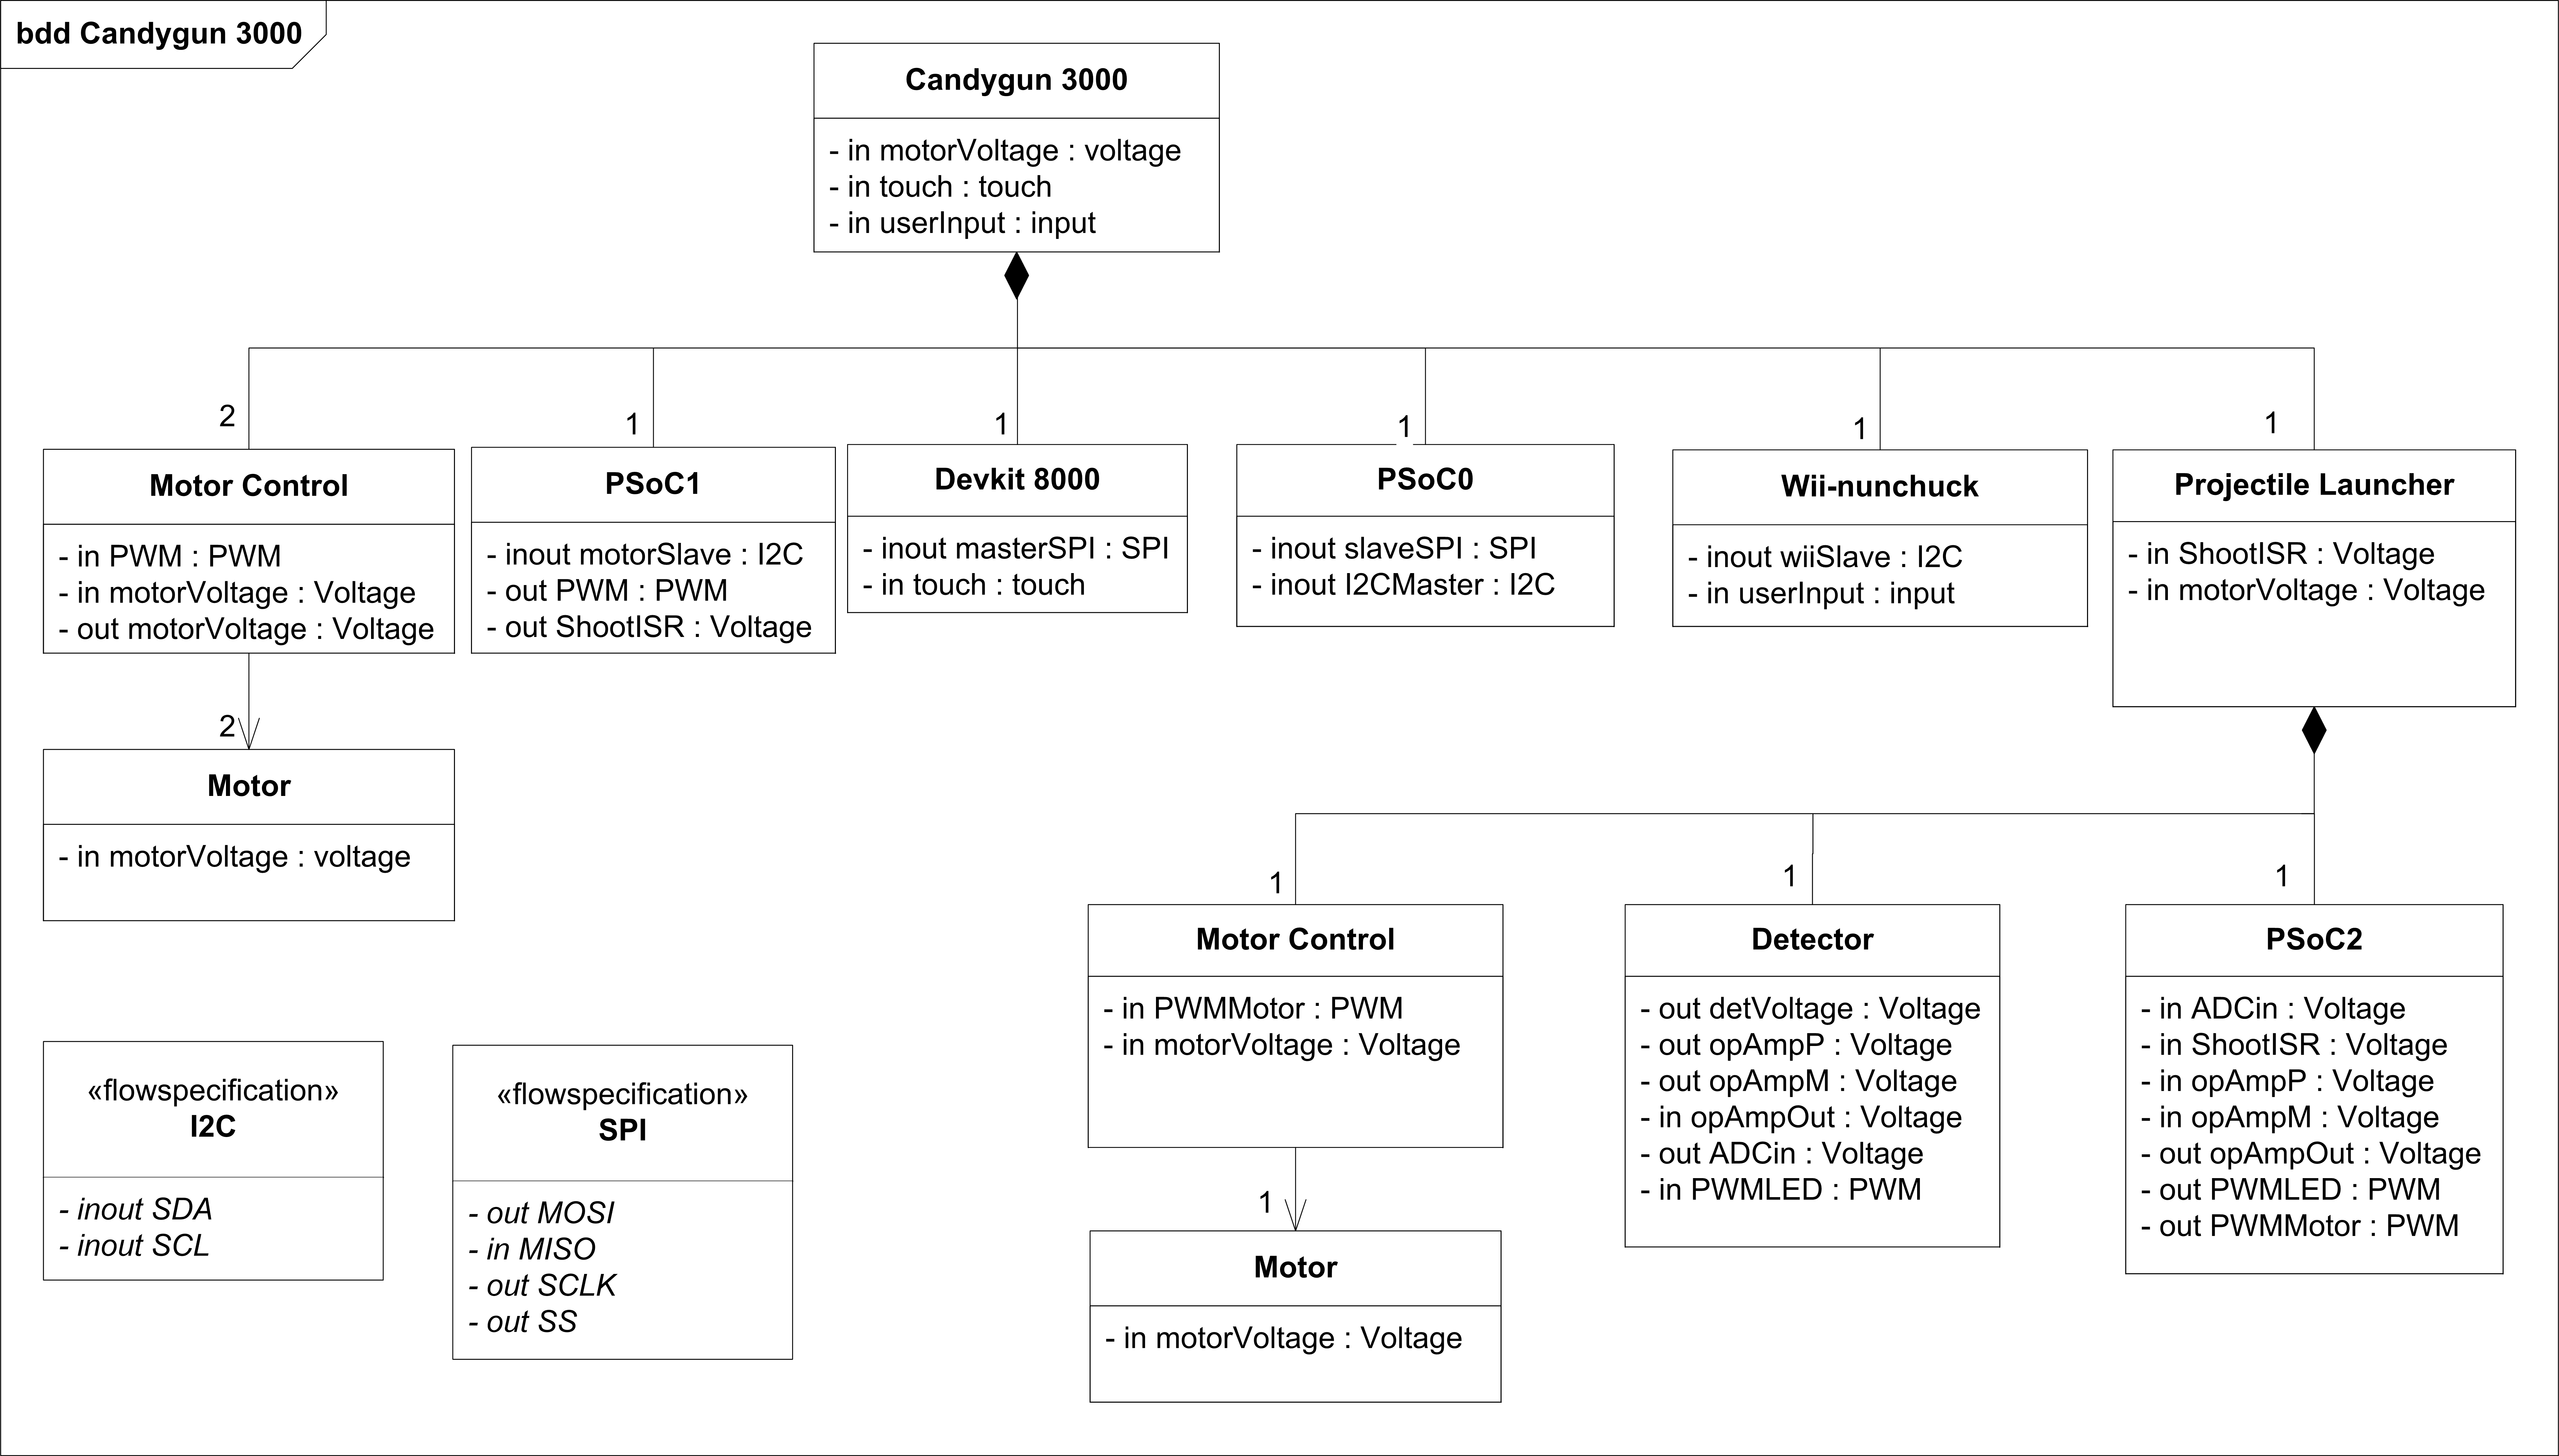
\includegraphics[width=0.85\paperwidth]{SystemArkitektur/images/BDD_overordnet1}
	\caption{BDD for systemets hardware}
	\label{figure:bddDiagram}
	\end{adjustwidth}
\end{figure}

\noindent På figur \ref{figure:bddDiagram} vises alle hardwareblokke fra domænemodellen (figur \ref{figure:domainModel}) med nødvendige indgange og udgange for de fysiske signaler. Yderligere ses det, at flowspecifikationer er defineret for de ikkeatomare forbindelser \textit{I2C}\cite{i2cbus} \cite{I2C} og \textit{SPI} \cite{spibus}, da disse er busser bestående af flere forbindelser.

\subsection{Blokbeskrivelse}
Følgende afsnit indeholder en blokbeskrivelse samt en flowspecifikation for I2C og SPI. I flowspecifikationen beskrives signalerne for I2C og SPI busserne.  I blokbeskrivelsen beskrives hver enkelt blok, så der fås en ide om, hvad hver blok består af, hvis de består af flere ting. Derudover skal det give et overblik over, hvad hver blok bruges til i systemet. \newline \newline

\begin{table}[H]
	\centering
	\begin{tabular}{|l|l|}
		\hline
		\textbf{Bloknavn}       & \textbf{Beskrivelse}                                                                                                                                                                                                                           \\ \hline
		Devkit 8000             & \begin{tabular}[c]{@{}l@{}}
		DevKit 8000 er en embedded linuxplatform med touchskærm, \\ der bruges til brugergrænsefladen for produktet. Brugeren inter- \\ agerer med systemet og ser status for spillet via Devkit 8000.                                                      \end{tabular} \\ \hline
		Wii-Nunchuck            & \begin{tabular}[c]{@{}l@{}}Wii-Nunchuck er controlleren, som brugeren styrer kanonens \\ retning med. \end{tabular} \\ \hline
		PSoC0                   & \begin{tabular}[c]{@{}l@{}}PSoC0 indeholder software til I2C og \\ SPI kommunikationen og afkodning af Wii-Nunchuck data. \\ PSoC0 fungerer som I2C master og SPI slave. Denne PSoC er \\ bindeleddet mellem brugergrænsefladen og resten af systemets \\ hardware. \end{tabular} \\ \hline
		Motor Control                   & \begin{tabular}[c]{@{}l@{}}Motor Control blokken er Candy Gun 3000’s motorer, der anvendes \\ til at bevæge kanonen. Denne blok består af H-bro-blokken og \\ rotationsbegrænsningsblokken. \end{tabular} \\ \hline
		Motor &
		\begin{tabular}[c]{@{}l@{}}Motor er motorene, der bruges til at bevæge platform og kanon. \end{tabular} \\ \hline
		H-bro &
		\begin{tabular}[c]{@{}l@{}}H-bro bruges til at styre motorens rotationsretning. \end{tabular} \\ \hline
		Rotationsbegrænsning &
		\begin{tabular}[c]{@{}l@{}}Rotationsbegrænsning er til at begrænse platformens rotation så \\ den ikke kan dreje 360 grader. Den blok består af et potentiometer \\ og en ADC, som sidder internt på PSoC0.  \end{tabular} \\ \hline
		PSoC1                   & \begin{tabular}[c]{@{}l@{}}PSoC1 indeholder software til I2C- \\ kommunikation og styring af Candy Gun 3000’s motorer. \\ PSoC1 fungerer som I2C slave. \end{tabular} \\ \hline
		SPI (FlowSpecification) &  \begin{tabular}[c]{@{}l@{}}SPI (FlowSpecification) beskriver signalerne der indgår i SPI \\ bussen. En fuld beskrivelse af bussen kan ses i dokumentationen \\ afsnit 3.7.1-\textit{SPI Protokol} side 44 \end{tabular} \\ \hline
		I2C (FlowSpecification) &  \begin{tabular}[c]{@{}l@{}}I2C (FlowSpecification) beskriver signalerne der indgår i I2C \\ bussen. En fuld beskrivelse af bussen kan ses i dokumentationen \\ afsnit 3.7.2-\textit{I2C Protokol} side 46 \end{tabular} \\ \hline	
		Projectile Launcher  &  \begin{tabular}[c]{@{}l@{}} Affyringsmekanismen indeholder PSoC2, Motor Control Shoot, \\ Motor Shoot og Rotation Detector og sørger dermed for \\ affyring af kanonen.  \end{tabular} \\ \hline
		PSoC2  & \begin{tabular}[c]{@{}l@{}} PSoC2 indeholder en operationsforstærker til rotations-\\detektorkredsløbet og en ADC som aflæser rotationsdetektoren. \\ Derudover står den for at sende PWM-signaler til LED'en \\ i rotationsdetektoren og til motorstyringsblokken.   \end{tabular} \\ \hline
		Motor Control Shoot  &  \begin{tabular}[c]{@{}l@{}} Denne blok står for at styre affyringsmekanismens motor.  \end{tabular} \\ \hline
		Motor Shoot  &  \begin{tabular}[c]{@{}l@{}} Motor Shoot er motoren, der sidder i affyringsmekanismen.  \end{tabular} \\ \hline
		Rotation Detector  &  \begin{tabular}[c]{@{}l@{}} Rotationsdetekoren detekterer, at der er blevet affyret et stykke \\ slik og sender et signal til PSoC2 om dette. \end{tabular} \\ \hline
	\end{tabular}
	\label{blokbeskrivelse}
	\caption{Blokbeskrivelse for BDD'et}
\end{table}

\subsection{IBD}
\label{afsnit:IBD}

På figur \ref{figure:ibdDiagram} ses IBD'et for systemet. Figuren viser hardwareblokkene med de fysiske forbindelser beskrevet i BDD'et, som ses på (figur \ref{figure:bddDiagram}). 

\begin{figure}[H]
	\begin{adjustwidth}{-3cm}{-\rightmargin}
	\centering
	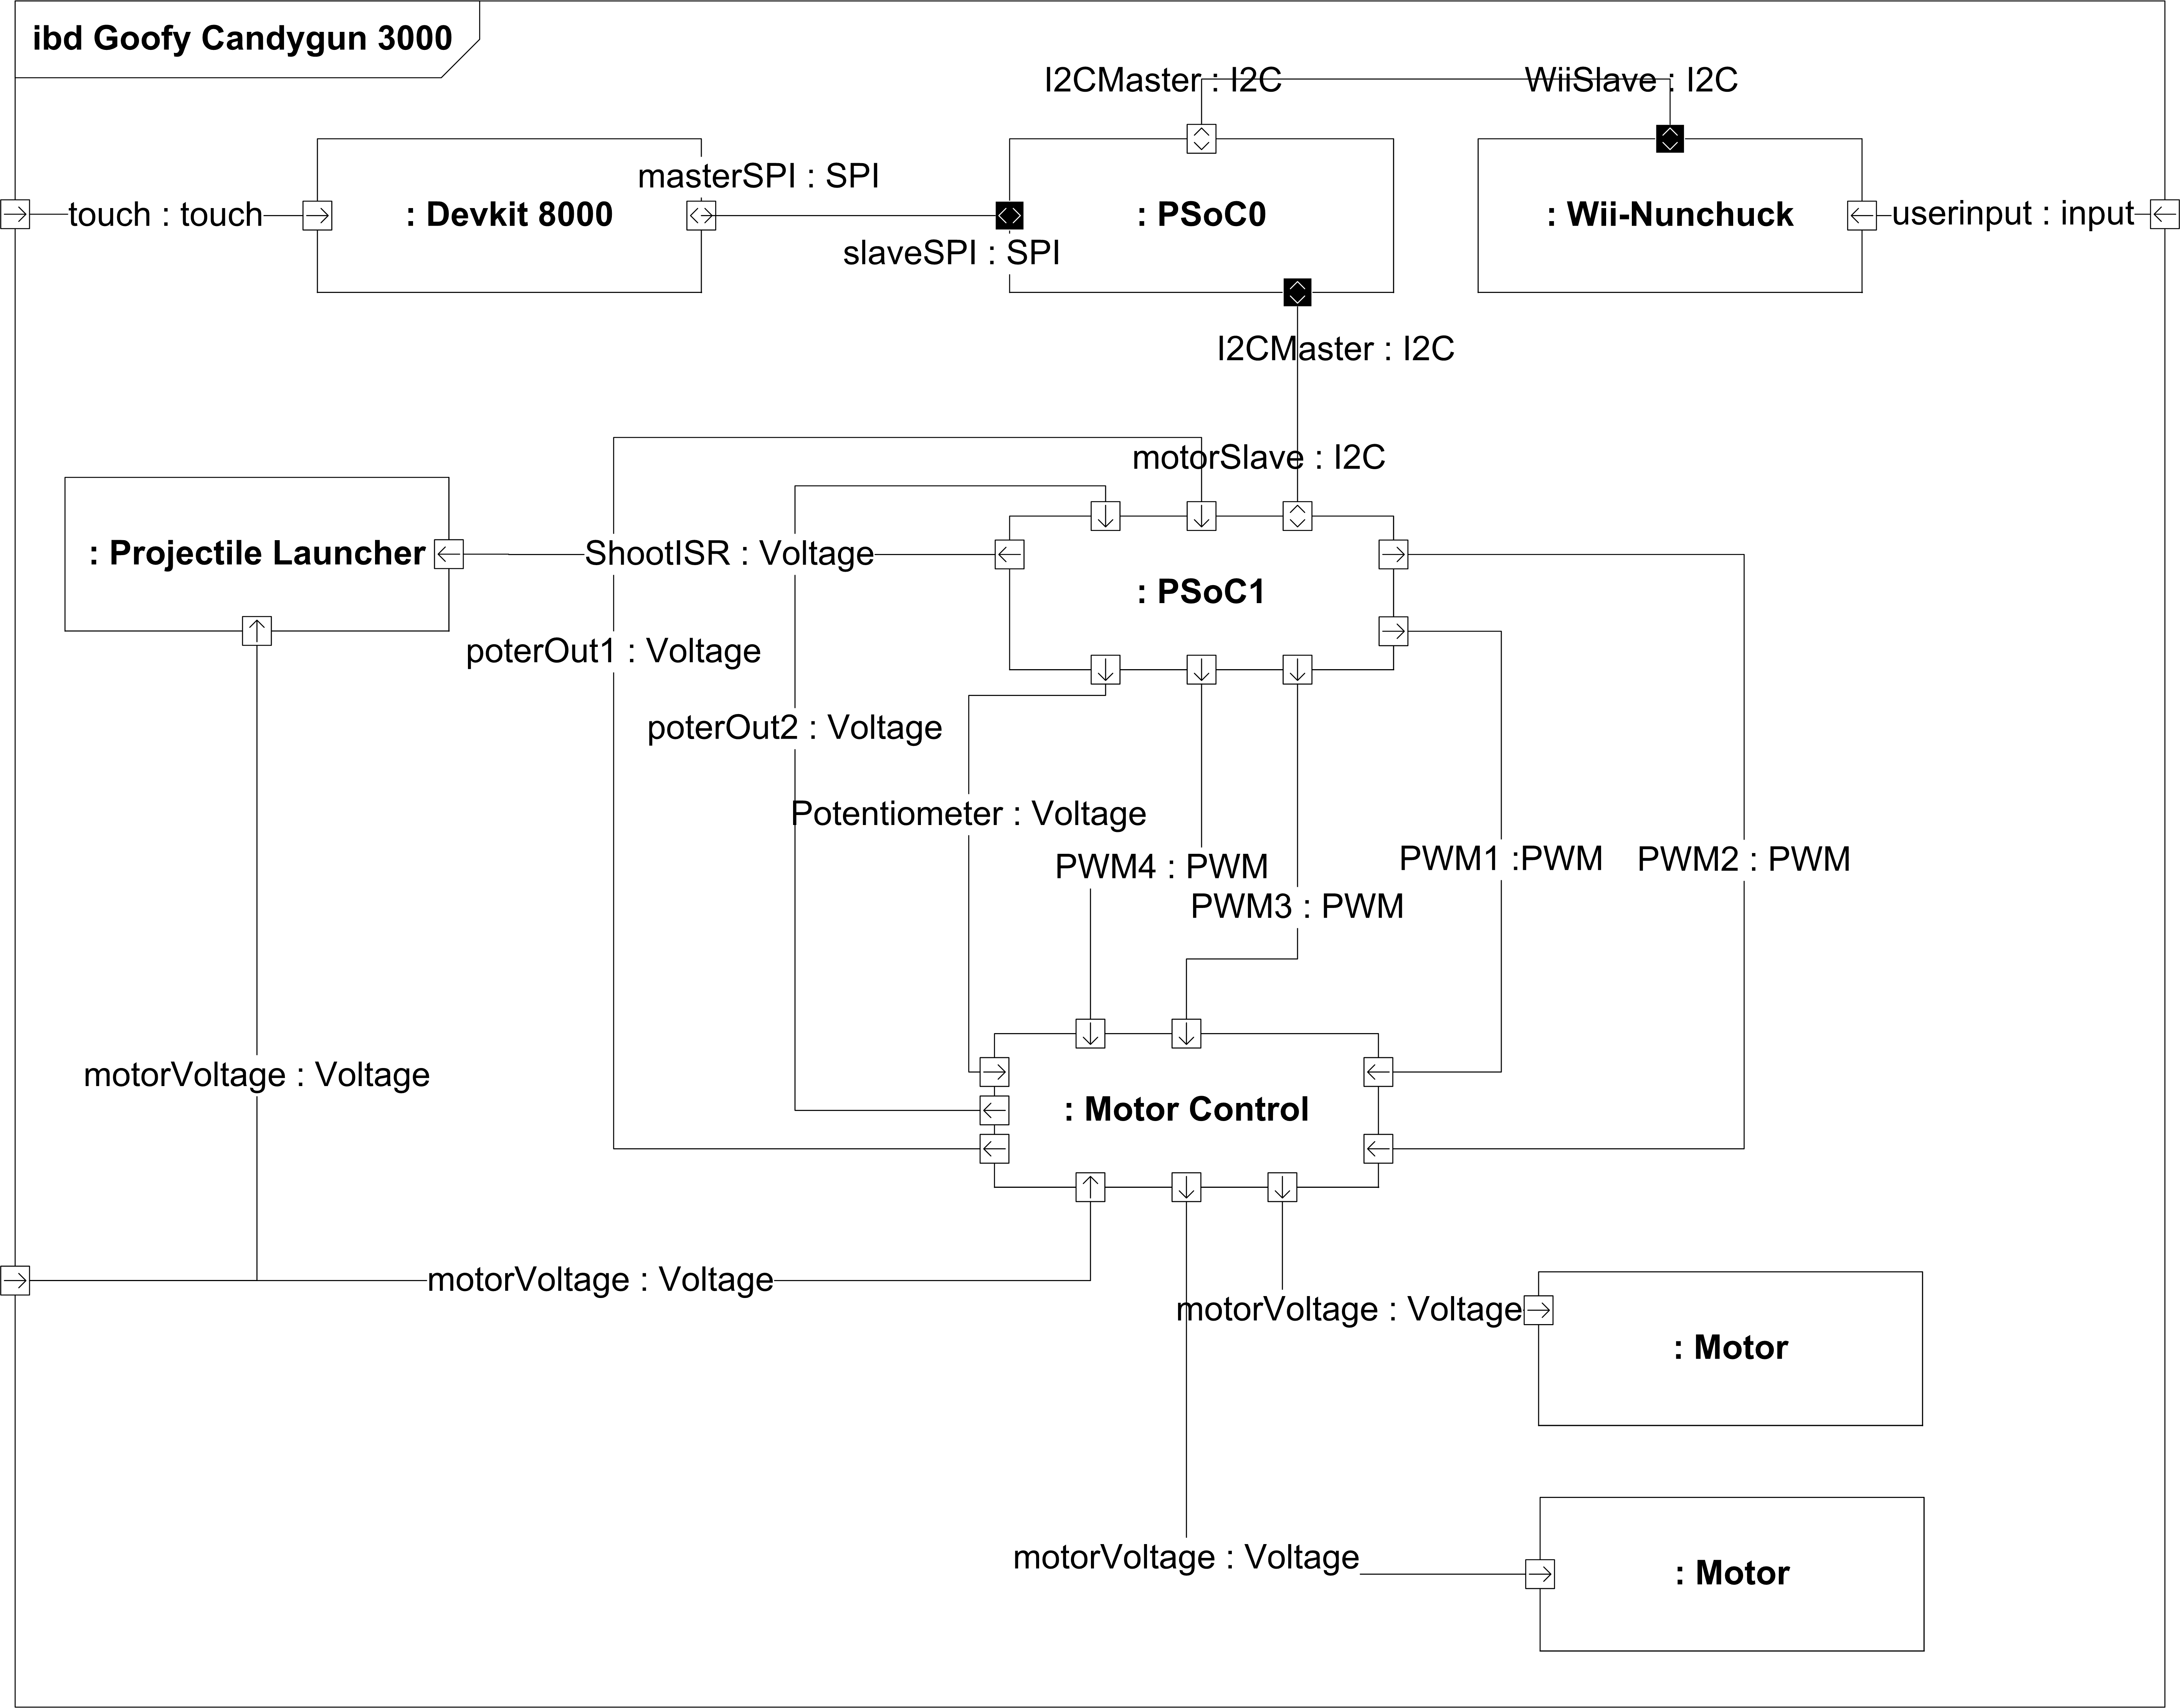
\includegraphics[width=0.85\paperwidth]{SystemArkitektur/images/IBD_V4}	
	\caption{IBD for systemets hardware}
	\label{figure:ibdDiagram}
	\end{adjustwidth}
\end{figure} 

\noindent Det ses, at systemet bliver påvirket af tre eksterne signaler: \textit{touch}, \textit{userinput}, samt \textit{motorVoltage}. \textit{touch} er input fra brugeren, når der interageres med brugergrænsefladen. \textit{userinput} er brugerens interaktion med Wii-Nunchuk. \textit{motorVoltage} er forsyningsspænding til systemet.\newline

\noindent I tabel \ref{table:signalbeskrivelse} ses beskrivelser af alle signaler i systemet. Et mere detaljeret IBD for hardwareenhederne \textit{Projectile Launcher} og \textit{Motor Control} kan ses i dokumentationen afsnit 3.3 - \textit{IBD for Candy Gun 3000} side 13. 

\newpage
\subsection{Signalbeskrivelse}
\begin{longtable}{|>{\hspace{0pt}}p{3cm} | >{\hspace{0pt}}p{3cm} | p{2cm} | p{3cm} |}
	\hline 
	                        
	\textbf{Blok-navn} & \textbf{Funktionsbeskrivelse} & \textbf{Signaler} & \textbf{Signalbeskrivelse} \\ \hline
	Devkit 8000 & Fungerer som grænseflade mellem bruger og systemet samt SPI master. & masterSPI & Type: SPI \newline Spændingsniveau: 0-5V \newline Hastighed: 1Mbps \newline Beskrivelse: SPI bussen hvori der sendes og modtages data.\\ \cline{3-4}
	& & touch & Type: touch \newline Beskrivelse: Brugertryk på Devkit 8000 touchdisplay. \\ \hline
	PSoC0 & Fungerer som I2C master for PSoC1 og Wii-Nunchuck samt SPI slave til Devkit 8000. & slaveSPI & Type: SPI \newline Spændingsniveau: 0-5V \newline Hastighed: 1Mbps \newline Beskrivelse: SPI bussen hvori der sendes og modtages data.\\ \cline{3-4}
	& & wiiMaster & Type: I2C \newline Spændingsniveau: 0-5V\newline Hastighed: 100kbps \newline Beskrivelse: I2C bussen hvor der modtages data fra Nunchuck.\\ \cline{3-4}
	& & motorMaster & Type: I2C \newline Spændingsniveau: 0-5V \newline Hastighed: 100kbps \newline Beskrivelse: I2C bussen hvor der sendes afkodet Nunchuck data til PSoC1.\\ \hline
	
	PSoC1 & Modtager nunchuckinput fra PSoC0 og omsætter dataene til PWM signaler. & motorSlave & Type: I2C \newline Spændingsniveau: 0-5V \newline Hastighed: 100kbps \newline Beskrivelse: Indeholder formatteret Wii-Nunchuck data, som omsættes til PWM-signal. \\ \cline{3-4} 
	&& ShootISR & Type: voltage \newline Spændingsniveau: 0-5V \newline Beskrivelse: Giver et højt signal, når den skal skyde.\\ \cline{3-4} 
	& & PWM & Type: PWM \newline Frekvens: 22kHz \newline PWM \%: 0-100\% \newline Spændingsniveau: 0-5V \newline Beskrivelse: PWM signal til styring af motorens hastighed. \\ \cline{3-4}
	& & PotenOut1 & Type: Voltage \newline Spændingsniveau: 0V-5V \newline Beskrivelse: Den spænding, der viser, hvor motoren står henne\\ \cline{3-4}
	& & PotenOut2 & Type: Voltage \newline Spændingsniveau: 0V-5V \newline Beskrivelse: Den spænding, der viser, hvor motoren står henne. \\ \cline{3-4}
	& & PWM1 & Type: PWM \newline Frekvens: 3MHz \newline PWM\%: 0-100\% \newline Spændingsniveau: 0-5V \newline Beskrivelse: PWM-signal til styring af motorens hastighed. \\ \cline{3-4}
	&& PWM2 & Type: PWM \newline Frekvens: 3MHz \newline PWM\%: 0-100\% \newline Spændingsniveau: 0-5V \newline Beskrivelse: PWM-signal til styring af motorens hastighed. \\ \cline{3-4}	
	&& PWM3 & Type: PWM \newline Frekvens: 3MHz \newline PWM\%: 0-100\% \newline Spændingsniveau: 0-5V \newline Beskrivelse: PWM-signal til styring af motorens hastighed. \\ \cline{3-4}
	&& PWM4 & Type: PWM \newline Frekvens: 3MHz \newline PWM\%: 0-100\% \newline Spændingsniveau: 0-5V \newline Beskrivelse: PWM-signal til styring af motorens hastighed. \\ \cline{3-4}
	& & motorVoltage & Type: Voltage \newline Spændingsniveau: 9V \newline Beskrivelse: Strømforsyning til motoren\\ \cline{3-4}
	& & potentiometer & Type: Voltage \newline Spændingsniveau: 5V \newline Beskrivelse: Giver Rotationsbegrænsing 5V. \\ \hline
	
	MotorControl & Den enhed, der skal bevæge kanonen. & PWM1 & Type: PWM \newline Frekvens: 3MHz \newline PWM\%: 0-100\% \newline Spændingsniveau: 0-5V \newline Beskrivelse: PWM-signal til styring af motorens hastighed. \\ \cline{3-4}
	&& PWM2 & Type: PWM \newline Frekvens: 3MHz \newline PWM\%: 0-100\% \newline Spændingsniveau: 0-5V \newline Beskrivelse: PWM-signal til styring af motorens hastighed. \\ \cline{3-4}
	&& PWM3 & Type: PWM \newline Frekvens: 3MHz \newline PWM\%: 0-100\% \newline Spændingsniveau: 0-5V \newline Beskrivelse: PWM-signal til styring af motorens hastighed. \\ \cline{3-4}
	&& PWM4 & Type: PWM \newline Frekvens: 3MHz \newline PWM\%: 0-100\% \newline Spændingsniveau: 0-5V \newline Beskrivelse: PWM-signal til styring af motorens hastighed. \\ \cline{3-4}
	& & motorVoltage & Type: Voltage \newline Spændingsniveau: 9V \newline Beskrivelse: Strømforsyning til motoren\\ \cline{3-4}
	& & potentiometer & Type: Voltage \newline Spændingsniveau: 5V \newline Beskrivelse: Giver Rotationsbegrænsing 5V. \\ \cline{3-4}
	& & PotenOut1 & Type: Voltage \newline Spændingsniveau: 0V-5V \newline Beskrivelse: Den spænding, der viser, hvor motoren står henne. \\ \cline{3-4}
	& & PotenOut2 & Type: Voltage \newline Spændingsniveau: 0V-5V \newline Beskrivelse: Den spænding, der viser, hvor motoren står henne. 
	\\ \hline
	
	Motor & Denne blok beskriver, hvad motoren får. & motorVoltage & Type: Voltage \newline Spændingsniveau: 0-5V  \newline Beskrivelse: Giver spænding til motoren. Gælder for begge. \\ \hline
	
	Wii-nunchuck & Den fysiske controller, som brugeren styrer kanonen med. & wiiSlave & Type: I2C \newline Spændingsniveau: 0-5V \newline Hastighed: 100kbps \newline Beskrivelse: Kommunikationslinje mellem PSoC1 og Wii-Nunchuck. \\ \cline{3-4}
	& & userInput & Type: input \newline Beskrivelse: Brugerinput fra Wii-Nunchuck. \\ \hline
	
	SPI & Denne blok beskriver den ikkeatomiske SPI-forbindelse. & MOSI & Type: CMOS \newline Spændingsniveau: 0-5V \newline Beskrivelse: Binært data, der sendes fra master til slave. \\ \cline{3-4}
	& & MISO & Type: CMOS \newline Spændingsniveau: 0-5V \newline Beskrivelse: Binært data, der sendes fra slave til master. \\ \cline{3-4}
	& & SCLK & Type: CMOS \newline Spændingsniveau: 0-5V \newline Hastighed: 1Mbps\newline Beskrivelse: clocksignalet fra master til slave, som bruges til at synkronisere den serielle kommunikation. \\ \cline{3-4}
	& & SS & Type: CMOS \newline Spændingsniveau: 0-5V \newline  Beskrivelse: Slave-Select, som bruges til at bestemme, hvilken slave der skal kommunikeres med. \\ \hline
	
	I2C & Denne blok beskriver den ikkeatomiske I2C-forbindelse. & SDA & Type: CMOS \newline Spændingsniveau: 0-5V \newline Beskrivelse: Databussen mellem I2C master og I2C slaver. \\ \cline{3-4}
	& & SCL & Type: CMOS \newline Spændingsniveau: 0-5V \newline Hastighed: 100kbps \newline Beskrivelse: Clock signalet fra master til lyttende I2C slaver, som bruges til at synkronisere den serielle kommunikation. \\ \hline
	
	Projectile Launcher & Denne blok består blokkene PSoC2, Detector og Motor Control Shoot & shootISR & Type: Voltage \newline Spændingsniveau: 0-5V \newline \newline Beskrivelse: Giver et højt signal, når kanonen skal skyde. \\ \cline{3-4}
	& & motorVoltage & Type: Voltage \newline Spændingsniveau: 9V \newline Beskrivelse: Strømforsyning til motor.  \\ \hline
	
	PSoC2 & Aflæser signaler fra rotationsdetektor og udsender PWM-signal til LED og Motor Shoot. & ADCin & Type: Voltage \newline Spændingsniveau: 0,5-5V \newline Beskrivelse: Rotationsdetektors output, som aflæses af ADC på PSoC2.  \\ \cline{3-4}
	& & shootISR & Type: Voltage \newline Spændingsniveau: 0-5V \newline Beskrivelse: Giver et højt signal, når motoren skal skyde. \\ \cline{3-4}
	& & opAmpP & Type: Voltage \newline Spændingsniveau: 0,5V \newline Beskrivelse: Referencespænding til operationsforstærkerens positive indgang. \\ \cline{3-4}
	& & opAmpM & Type: Voltage \newline Spændingsniveau: 0,5V \newline Beskrivelse: Virtuelt nul. Den ligger altid på 0,5V pga. negativ feedback på operationsforstærkeren. \\ \cline{3-4}
	& & opAmpOut & Type: Voltage \newline Spændingsniveau: 0,5-5V \newline Beskrivelse: Udgang på operationsforstærker i rotationsdetektorkredsløbet. \\ \cline{3-4}
	& & PWMLED & Type: PWM \newline Spændingsniveau: 0-5V \newline Frekvens: 10kHz \newline PWM\%: 0-100\% \newline Beskrivelse: Udsender PWM-signal til LED'en i rotationsdetektorkredsløbet. \\ \cline{3-4}
	& & PWMMotor & Type: PWM \newline Spændingsniveau: 0-5V \newline Frekvens: 33,33kHz \newline PWM\%: 0-100\% \newline Beskrivelse: Udsender PWM-signal til LED'en i rotationsdetektorkredsløbet. \\ \hline
	
	Detector & Rotationsdetektoren detekterer om der er skudt. & opAmpP & Type: Voltage \newline Spændingsniveau: 0,5V \newline Beskrivelse: Referencespænding til operationsforstærkerens positive indgang. \\ \cline{3-4}
	& & opAmpM & Type: Voltage \newline Spændingsniveau: 0,5V \newline Beskrivelse: Virtuelt nul. Den ligger altid på 0,5V pga. negativ feedback på operationsforstærkeren. \\ \cline{3-4}
	& & opAmpOut & Type: Voltage \newline Spændingsniveau: 0,5-5V \newline Beskrivelse: Udgang på operationsforstærker i rotationsdetektorkredsløbet. \\ \cline{3-4}
	& & ADCin & Type: Voltage \newline Spændingsniveau: 0,5-5V \newline Beskrivelse: Rotationsdektors output, som aflæses af ADC på PSoC2.  \\ \cline{3-4}
	& & PWMLED & Type: PWM \newline Spændingsniveau: 0-5V \newline Frekvens: 10kHz \newline PWM\%: 0-100\% \newline Beskrivelse: Udsender PWM-signal til LED'en i rotationsdetektorkredsløbet. \\ \hline
	
	Motor Control Shoot & Denne blok styrer Motor Shoot til affyringsmekanismen. & PWMMotor & Type: PWM \newline Spændingsniveau: 0-5V \newline Frekvens: 33,33kHz \newline PWM\%: 0-100\% \newline Beskrivelse: Udsender PWM-signal til LED'en i rotationsdetektorkredsløbet. \\ \cline{3-4}
	& & motorVoltage & Type: Voltage \newline Spændingsniveau: 9V \newline Beskrivelse: Strømforsyning til motor. \\ \hline 
	
	Motor Shoot & Denne blok er affyringsmekanismens motor. & motorVoltage & Type: Voltage \newline Spændingsniveau: 9V \newline Beskrivelse: Strømforsyning til motor. \\ \hline
	\caption{Signalbeskrivelse}
	\label{table:signalbeskrivelse}
\end{longtable}

\section{Software}

\subsection{Softwareallokering}
\label{afsnit:SoftwareAllokering}

Domænemodellen i figur \ref{figure:domainModel}, side \pageref{figure:domainModel}, præsenterer systemets hardwareblokke. På figur \ref{figure:allocationDiagram} ses et software allokeringsdiagram, som viser på hvilke hardwareblokke de forskellige softwaredele er allokeret. 

\begin{figure}[H]
	\centering
	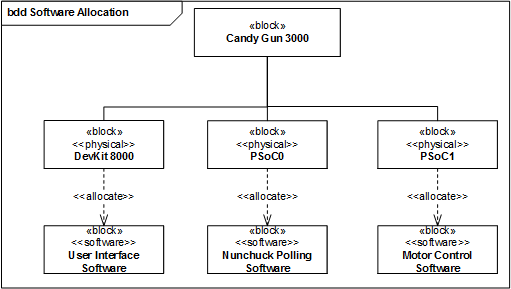
\includegraphics[width=\textwidth]{SystemArkitektur/images/SoftwareAllocation}
	\caption{Systemets softwareallokeringer}
	\label{figure:allocationDiagram}
\end{figure}

\noindent På figur \ref{figure:allocationDiagram} ses, at systemet består af fire primære softwaredele: \textit{User Interface Software}, \textit{Nunchuck Polling Software}, \textit{Motor Control Software} og \textit{Projectile Launcher Software}. Disse er fordelt over de fire viste CPU'er.\newline

\noindent I tabel \ref{tabel:softwareAllocationDescription} er hver allokeret softwarekomponent beskrevet.

\begin{table}[H]
	\centering
	\begin{tabular}{|ll|}
		\hline
		User Interface Software   & \begin{tabular}[c]{@{}l@{}}Dette allokerede software er brugergrænsefladen\\ som brugeren interagerer med på DevKit8000 touch-skærmen.\end{tabular}                                                  \\
		\rowcolor[HTML]{CBCEFB} 
		Nunchuck Polling Software & \begin{tabular}[c]{@{}l@{}}Dette allokerede software har til ansvar at polle\\ Nunchuck tilstanden og videresende det til\\ PSoC1.\end{tabular}                                                      \\
		Motor Control Software    & \cellcolor[HTML]{FFFFFF}\begin{tabular}[c]{@{}l@{}}Dette allokerede software har til ansvar at\\ bruge den pollede Nunchuck data fra PSoC0\\ til motorstyring samt affyringsmekanismen.\end{tabular} 
		\\ 
		\rowcolor[HTML]{CBCEFB} 
		Projectile Launcher Software & \begin{tabular}[c]{@{}l@{}}Dette allokerede software har til ansvar at aktivere\\ affyringsmekanismen når et \\ knaptryk detekteres på Nunchuck.\end{tabular} \\
		\hline
	\end{tabular}
	\caption{Beskrivelse af den allokerede software}
	\label{tabel:softwareAllocationDescription}
\end{table}

\subsection{Informationsflow i systemet}
\label{afsnit:informationFlow}
Dette afsnit har til formål at demonstrere sammenhængen mellem softwaren på CPU'erne og resten af systemet samt at beskrive og identificere grænsefladerne brugt til kommunikation mellem dem. Yderligere vil klasseidentifikation også blive vist, hvor disse klasser vil specificeres i afsnit \ref{afsnit:nunchuckDI}, i Design og Implementering.

\subsubsection{Wii-Nunchuck Information Flow}
En essentiel del af use case 1 er at kunne styre motoren ved brug af Wii-Nunchuck controlleren. På figur \ref{fig:WiiNunchuckSekvensDiagram} vises gennemløbet af Wii-Nunchucks inputdata fra Wii-Nunchucken til motoren med de relevante CPU'er angivet. Her ses det, at inputdata fra Wii-Nunchuck kontinuert bliver aflæst af PSoC0. Det bemærkes her, at grænsefladen mellem PSoC0 og Wii-Nunchuck er en I2C bus. Efter at PSoC0 har aflæst inputdata, overføres det til PSoC1. Grænsefladen mellem disse to PSoC's er også en I2C bus. PSoC1 kan til slut oversætte modtaget inputdata til PWM-signaler til motorstyring samt affyring.

\begin{figure}[H]
	\centering
	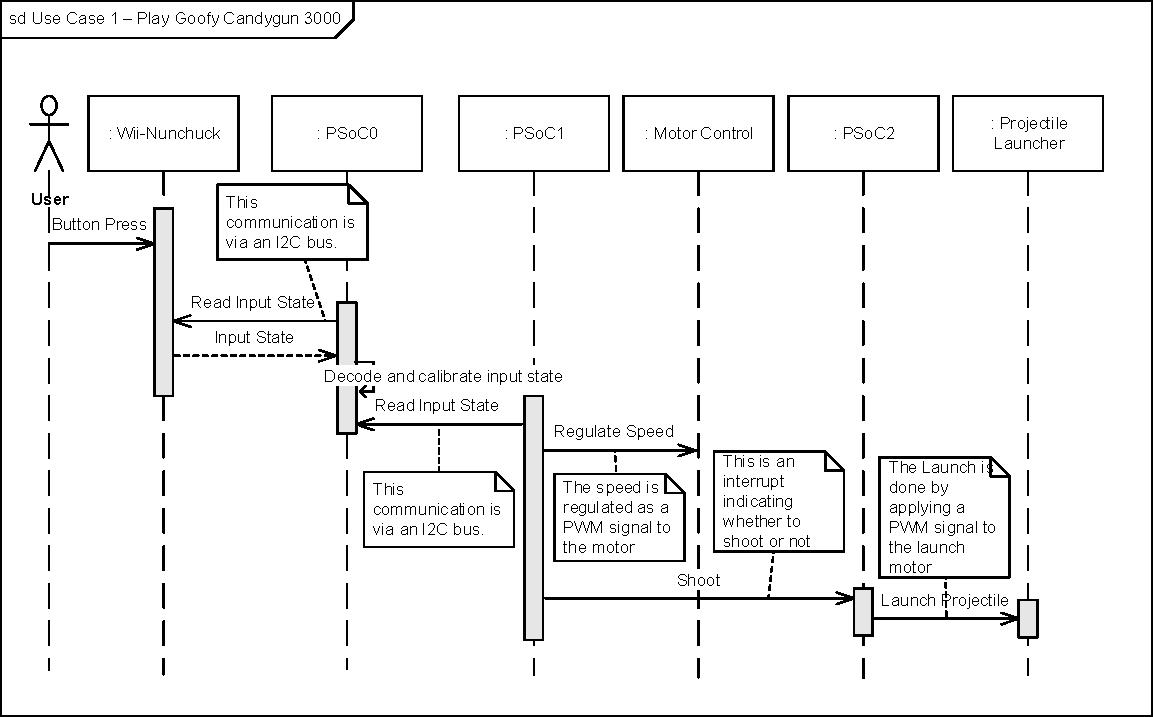
\includegraphics[width=\textwidth] {Systemarkitektur/images/SequenceDiagramUC1}
	\caption{Wii-Nunchuck Input Data Forløb}
	\label{fig:WiiNunchuckSekvensDiagram}
\end{figure}

\subsubsection{Systemtest}
Use case 2 beskriver test af systemet før spillet startes. På figur \ref{fig:SystemTestSekvensDiagram} vises testsekvensen for en vellykket test. 

\begin{figure}[H]
	\centering
	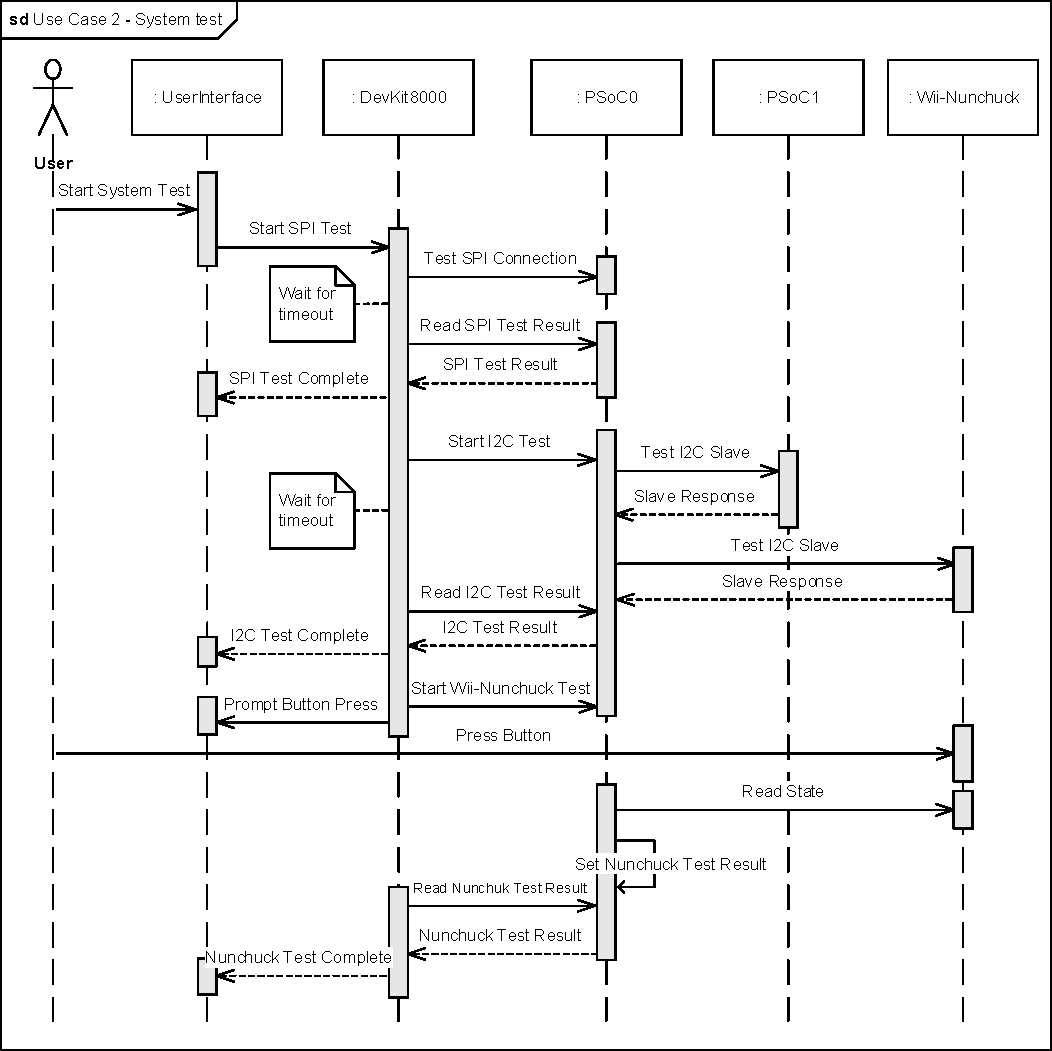
\includegraphics[width=\textwidth] {Systemarkitektur/images/SequenceDiagramUC2}
	\caption{System Test Forløb}
	\label{fig:SystemTestSekvensDiagram}
\end{figure}

\noindent Kommunikationen mellem Devkit 8000 og PSoC0 er initieret og styret af Devkit 8000. Da PSoC0 i dette design ikke har mulighed for at indikere, hvornår data er klar til aflæsning, skal Devkit 8000 vente på en \textit{timeout}, før den aflæser data på PSoC0. Dette er muligt, idet systemtesten bliver afviklet sekventielt.

\subsection{Samlede Klassediagrammer}
\label{afsnit:samledeKlasser}
På baggrund af sekvensdiagrammerne i afsnit \ref{afsnit:informationFlow} samt de detaljerede applikationsmodeller beksrevet i dokumentationen, afsnit 3.5-\textit{Applikationsmodeller} side 25, er der udledt samlede klassediagrammer for hver individuel CPU i systemet. Disse er med til at identificere konceptuelle klasser og funktionaliter, der skal overvejes i implementation og design af systemet og har altså fungeret som et udgangspunkt for resten af udviklingsprocessen. \newline

\noindent Figur \ref{fig:CompleteClassDiagramDevKit8000}, \ref{fig:CompleteClassDiagramPSoC0}, \ref{fig:CompleteClassDiagramPSoC1} og \ref{fig:CompleteClassDiagramPSoC2} viser de samlede klassediagrammer for hver CPU.\newline

\noindent For disse klassediagrammer er der konceptuelle klasser, som går igen på flere diagrammer. Alle klassediagrammer har én klasse af typen \textit{controller}. Disse klasser indeholder al funktionalitet, der er nødvendig for at kunne implementere systemets use cases. Derudover går klasserne \textit{I2C Interface} og \textit{SPI Interface} også igen på flere diagrammer. Disse repræsenterer klasser for de tilsvarende bustyper, I2C og SPI, og bruges af softwaren til at sende og modtage data på disse busser.\newline

\noindent På figur \ref{fig:CompleteClassDiagramDevKit8000} ses det, at Devkit 8000 controllerklassen skal have funktionalitet til start af systemtest i relation til use case 2. For at kunne udføre dette, kommunikerer den med grænsefladen Graphical User Interface (\textit{GUI}), og kan dermed vise resultater til brugeren. Desuden skal controlleren kommunikere med grænsefladen \textit{SPI Interface} for at sende data ud til resten af systemet via SPI bussen.

\begin{figure}[H]
	\centering
	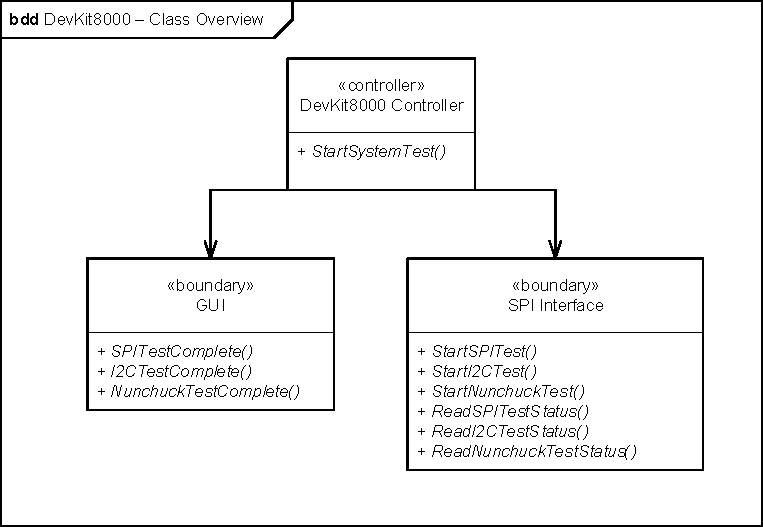
\includegraphics[width=\textwidth] {Systemarkitektur/images/CompleteClassDiagramDevKit8000}
	\caption{Samlet Klassediagram for Devkit 8000}
	\label{fig:CompleteClassDiagramDevKit8000}
\end{figure}

\noindent På figur \ref{fig:CompleteClassDiagramPSoC0} ses det, at PSoC0 controlleren skal have funktionalitet til at starte tests af systemets busser. Yderligere skal den også kunne aflæse, dekode og kalibrere data, der kommer fra Nunchuck. I relation til disse funktionaliteter skal den kunne modtage og sende data på systemets I2C og SPI busser.
\begin{figure}[H]
	\centering
	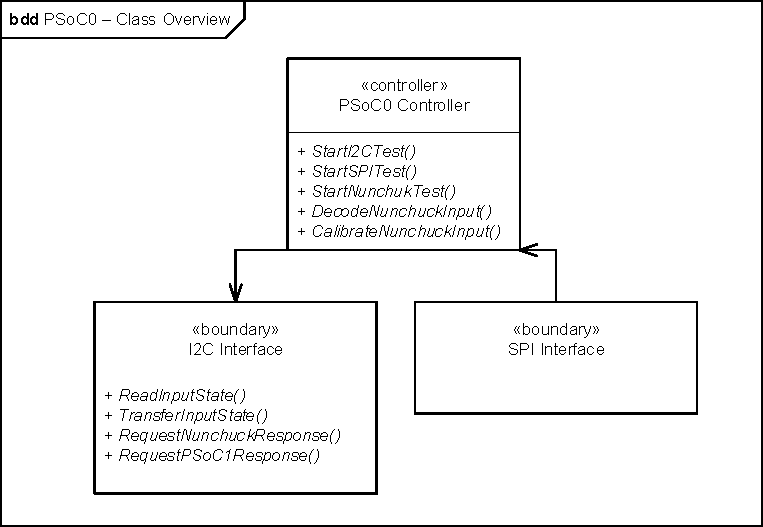
\includegraphics[width=\textwidth] {Systemarkitektur/images/CompleteClassDiagramPSoC0}
	\caption{Samlet Klassediagram for PSoC0}
	\label{fig:CompleteClassDiagramPSoC0}
\end{figure}

\noindent På figur \ref{fig:CompleteClassDiagramPSoC1} ses det, at PSoC1 controlleren kommunikerer med grænsefladerne \textit{I2C Interface}, \textit{Motor Control} samt \textit{PSoC2}. Controlleren skal kunne regulere hastighed på systemets motorstyring for at kunne styre kanonen. Desuden skal den kunne sende en affyringsbesked til \textit{PSoC2}. For at regulere hastighed og affyre kanonen, skal controlleren kunne aflæse Nunchucken's tilstand fra \textit{I2C Interface}.

\begin{figure}[H]
	\centering
	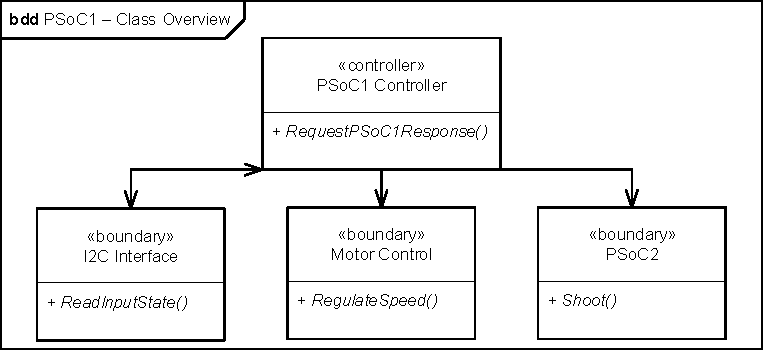
\includegraphics[width=\textwidth] {Systemarkitektur/images/CompleteClassDiagramPSoC1}
	\caption{Samlet Klassediagram for PSoC1}
	\label{fig:CompleteClassDiagramPSoC1}
\end{figure}

\noindent På figur \ref{fig:CompleteClassDiagramPSoC2} ses det, at PSoC2 skal have funktionalitet til at aktivere afskydning, som gøres ved at kommunikere med grænsefladen \textit{Projectile Launcher}. Afskydningen aktiveres af grænsefladen \textit{PSoC1}.
\begin{figure}[H]
	\centering
	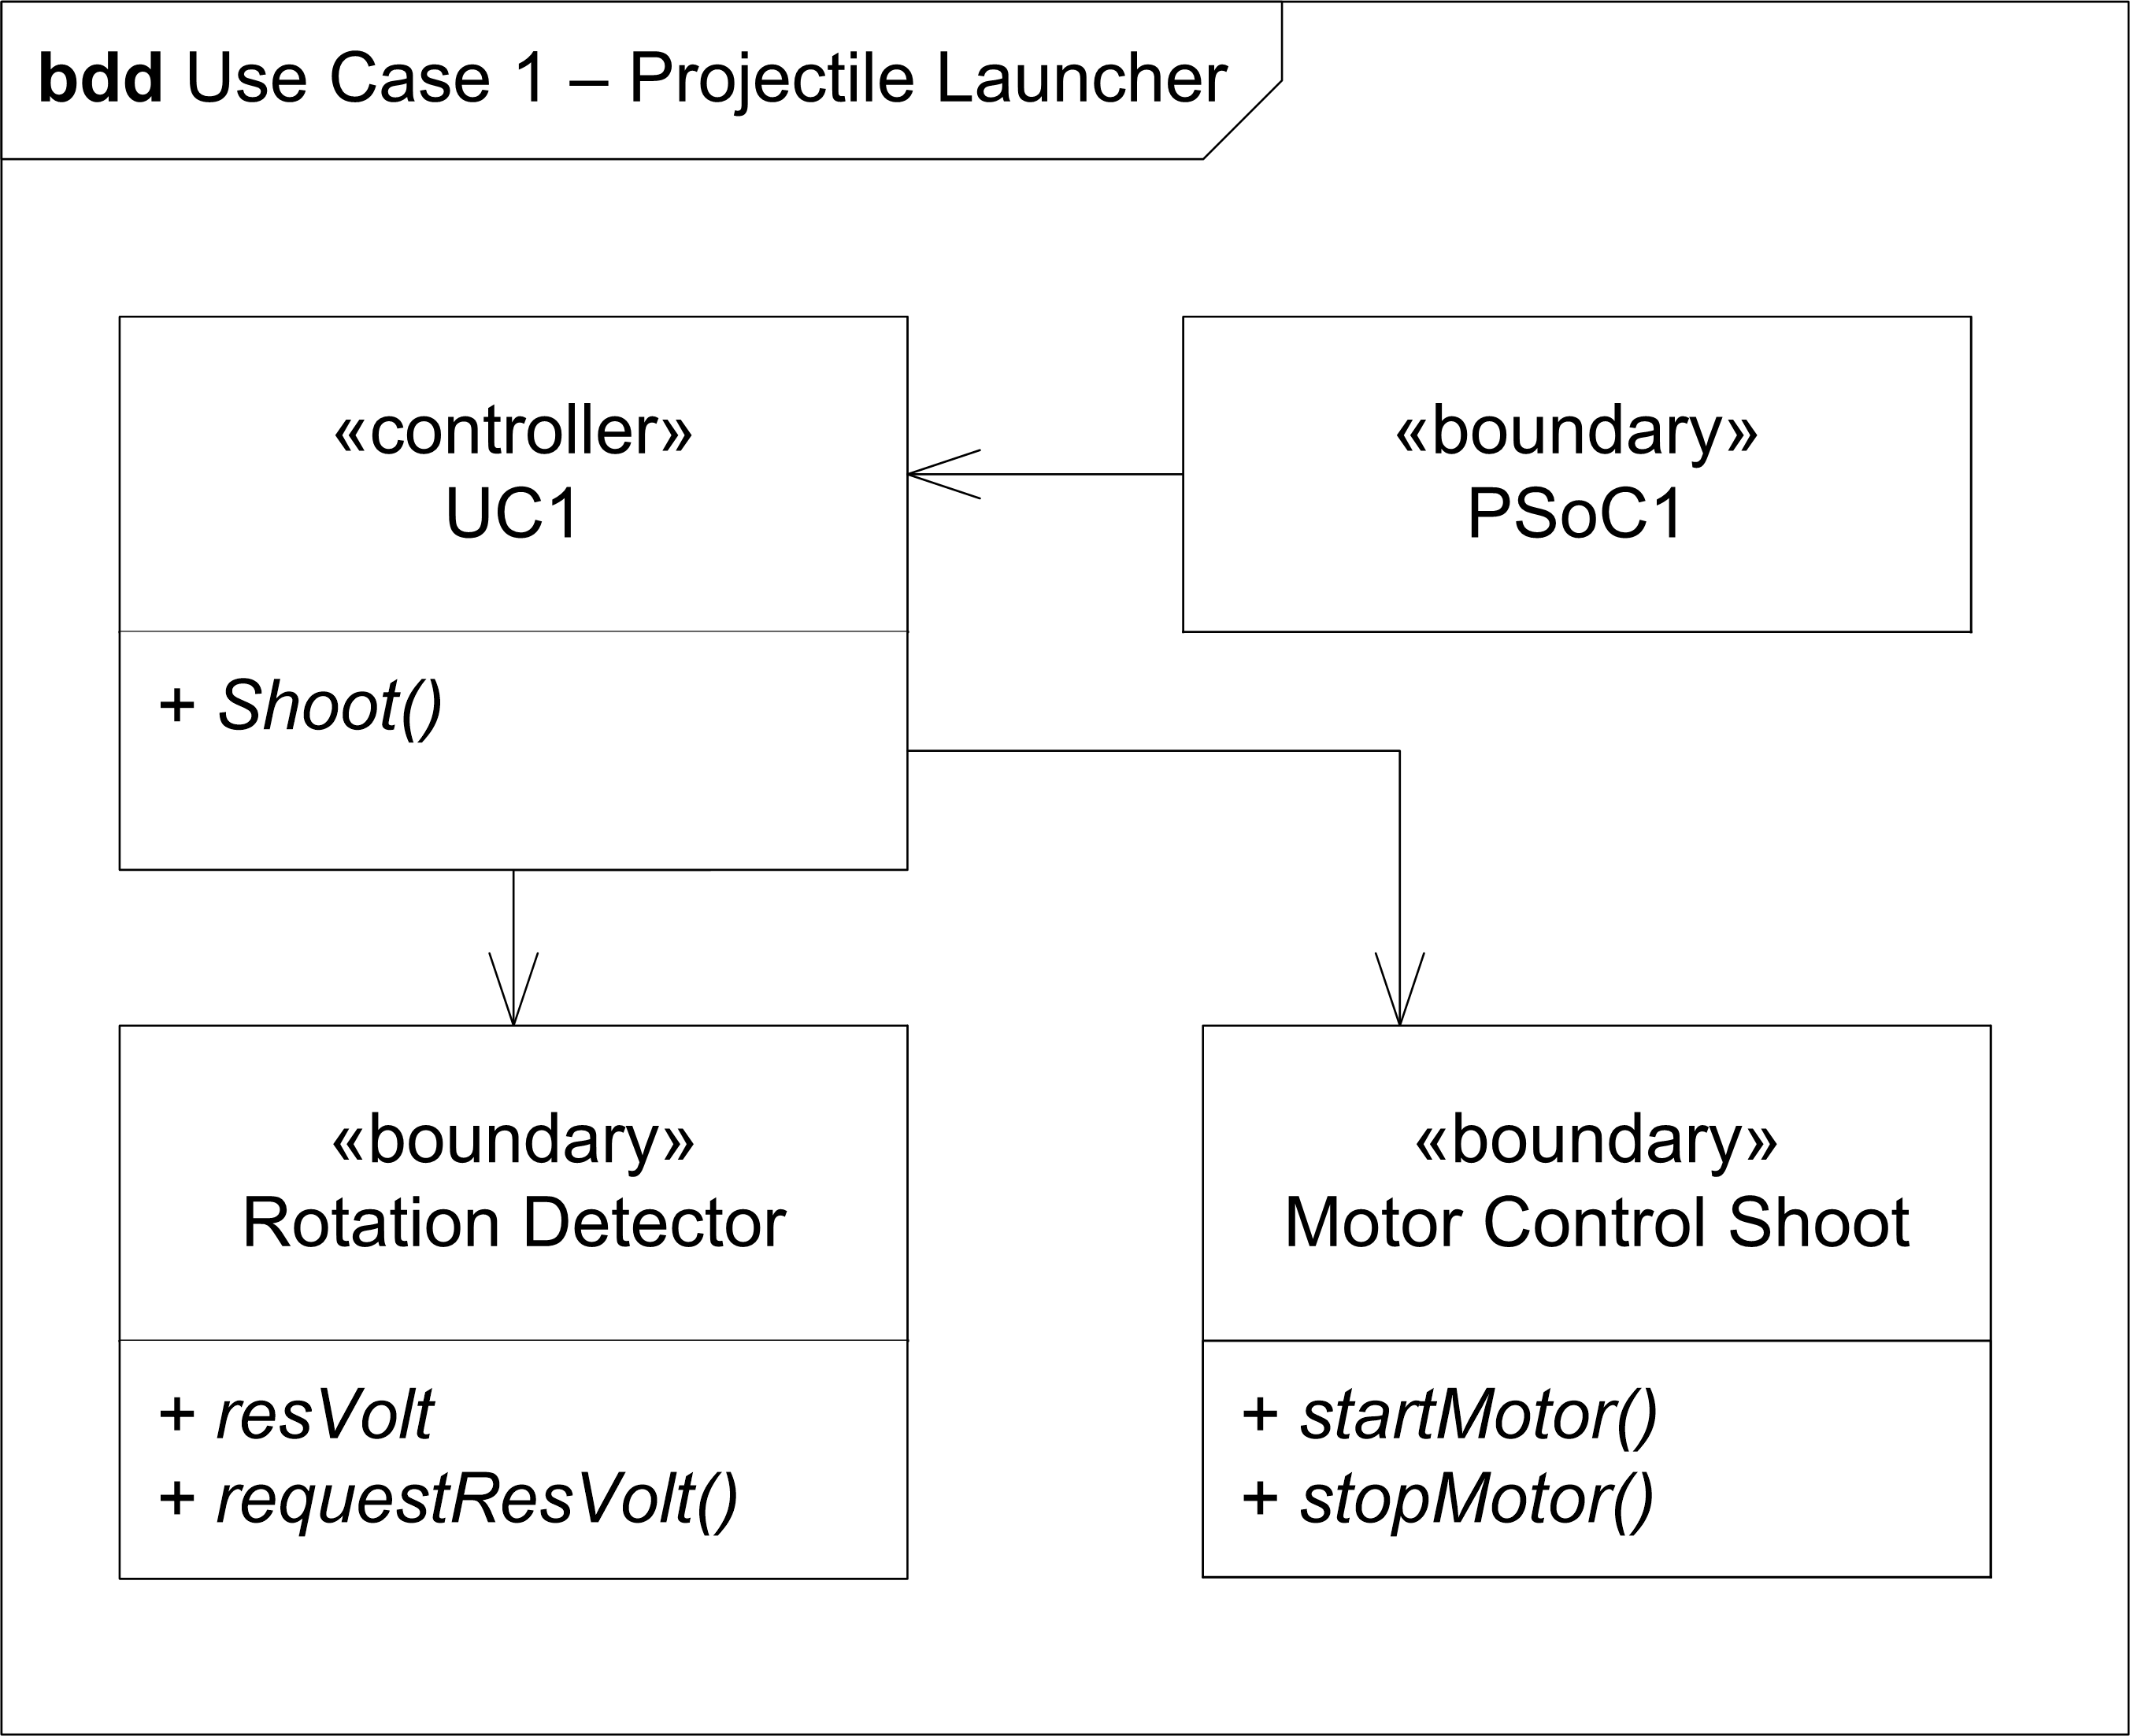
\includegraphics[width=\textwidth] {Systemarkitektur/images/affyringKlassediagram.png}
	\caption{Samlet Klassediagram for PSoC2}
	\label{fig:CompleteClassDiagramPSoC2}
\end{figure}

\subsection{SPI Kommunikations Protokol}
I afsnit \ref{afsnit:IBD}-IBD, ses på figur \ref{figure:ibdDiagram} at Devkit 8000 og PSoC0 kommunikerer via en SPI bus. Kommunikationen foregår ved at der sendes kommandotyper imellem de to enheder, SPI-master og SPI-slave. På tabel \ref{tabel:spiKommandoType} ses en de anvendte kommandotyper samt en kort beskrivelse for hver af disse. En fuld beskrivelse af SPI-kommunikations protokollen kan ses i dokumentationen afsnit 3.7.1-\textit{SPI Protokol} side 44.\newline

\noindent Der er til systemet valgt en SPI bus mellem Devkit 8000 og PSoC0, da der i dette tilfælde kun er brug for en bus med god support for én master og én slave. En SPI bus skalerer ikke godt med flere slaver i forhold til SPI, da en SPI bus skal have en fysisk forbindelse for hver enkelt slave, der tilkobles. Bussen er dog at implementere og er derfor ideel for denne grænseflade.

\begin{table}[H]
	\centering
	\resizebox{\textwidth}{!}{%
		\begin{tabular}{llll}
			\hline
			\multicolumn{1}{|l|}{Kommandotype}                                & \multicolumn{1}{l|}{Beskrivelse}                        & \multicolumn{1}{l|}{Binær Værdi} & \multicolumn{1}{l|}{Hex Værdi} \\ \hline
			\rowcolor[HTML]{CBCEFB} 
			{\color[HTML]{000000} START\_SPI\_TEST}                           & {\color[HTML]{000000} Sætter PSoC0 i 'SPI-TEST' mode}   & 1111 0001                        & 0xF1                           \\
			START\_I2C\_TEST                                                  & Sætter PSoC0 i 'I2C-TEST' mode                          & 1111 0010                        & 0xF2                           \\
			\rowcolor[HTML]{CBCEFB} 
			\begin{tabular}[c]{@{}l@{}}START\_NUN-\\ CHUCK\_TEST\end{tabular} & Sætter PSoC0 i 'NUNCHUCK-TEST' mode                     & 1111 0011                        & 0xF3                           \\
			SPI\_OK                                                           & Signalerer at SPI-testen blev gennemført uden fejl      & 1101 0001                        & 0xD1                           \\
			\rowcolor[HTML]{CBCEFB} 
			I2C\_OK                                                           & Signalerer at I2C-testen blev gennemført uden fejl      & 1101 0010                        & 0xD2                           \\
			I2C\_FAIL                                                         & Signalerer at I2C-testen fejlede           & 1100 0010                        & 0xC2                           \\
			\rowcolor[HTML]{CBCEFB} 
			NUNCHUCK\_OK                                                      & Signalerer at NUNCHUCK-testen blev gennemført uden fejl & 1101 0011                        & 0xD3                           \\
			NUNCHUCK\_FAIL                                                    & Signalerer at NUNCHUCK-testen fejlede      & 1100 0011                        & 0xC3                          
		\end{tabular}
	}
	\caption{SPI kommunikation kommandotyper}
	\label{tabel:spiKommandoType}
\end{table}

\noindent Kommandotyperne er udledt fra det samlede klassediagram for Devkit 8000, figur \ref{fig:CompleteClassDiagramDevKit8000}. På figuren kan det ses, at \textit{Devkit 8000 Controller} skal kunne starte tests for SPI, I2C samt Nunchuck og aflæse resultatet af disse. \newline

\noindent Kommunikation på en SPI-bus foregår ved bit-shifting. Dette betyder, at indholdet af masterens transfer buffer bliver skiftet over i slavens read buffer og omvendt. Kommunikationen foregår i fuld duplex, og derfor skal der foretages to transmissioner for at aflæse data fra en SPI-slave. Dette skyldes, at slaven skal vide hvilke data, der skal klargøres i transfer-bufferen og klargøre denne buffer før masteren kan aflæse denne. Her skal der tages højde for, at en længere proces skal gennemføres før slaven har klargjort transfer-bufferen. Derfor skal masteren efter at have sendt en kommandotype vente et bestemt stykke tid, før der aflæses fra slavens transfer-buffer. Denne sekvens er illustreret med et sekvensdiagram på figur \ref{figure:SDSpiSlaveRead}.

\begin{figure}[H]
	\centering
	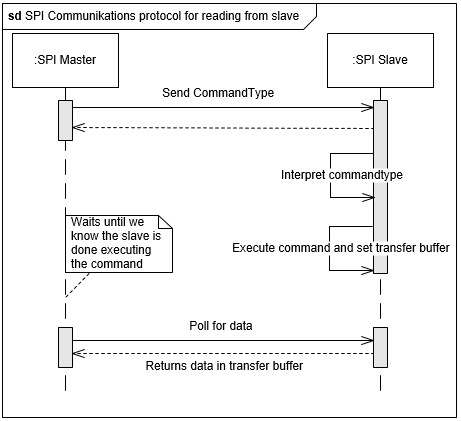
\includegraphics[]{Systemarkitektur/images/SDSpiSlaveRead}
	\caption{Sekvensdiagram for aflæsning data fra en SPI-slave}
	\label{figure:SDSpiSlaveRead}
\end{figure} 

\subsubsection{Designvalg}
SPI kommunikationsprotokollen er designet ud fra det grundlag, at Devkit 8000 som SPI master skal læse tilstande fra SPI slaven ved brug af en timeout model. Ved timeout model menes der, at Devkit 8000 sender en kommandotype ud, venter et bestemt antal sekunder, og herefter læser værdien fra SPI slaven. Denne model er modelleret på figur \ref{figure:SDSpiSlaveRead}.\newline

\noindent Et alternativt design ville være at generere et interrupt til SPI masteren når slaven havde data der skulle læses. Til dette system blev timeout modellen dog valgt, da det hardwaremæssigt var simplere at implementere, samt at al nødvendig funktionalitet kan implementeres med den valgte model.

\subsection{I2C Kommunikations Protokol}
\label{afsnit:I2CProtokol}
I afsnit \ref{afsnit:IBD}-\textit{IBD}, ses det på figur \ref{figure:ibdDiagram} at tre hardwareblokke kommunikerer via en I2C bus. Til denne I2C kommunikation er der defineret en protokol, som bestemmer hvordan modtaget data skal fortolkes. Denne protokol vil blive præsenteret her, men en fuld gennemgang kan findes i dokumentationen afsnit 3.7.2-\textit{I2C Protokol} side 46.\newline

\noindent I2C bussen er brugt til disse forbindelser af to primære grunde. Først og fremmest er Nunchuck controlleren implementeret som en I2C Slave fra producentens side. Derfor skulle der gøres brug af en I2C bus i alle tilfælde, for at kommunikere med Nunchucken. Yderligere skulle Nunchuken's input sendes videre til PSoC1, og I2C er en bus der skalerer godt med multiple enheder \cite{i2cbus}. Derfor var det naturligt at udvide I2C bussen mellem Nunchuck og PSoC0, med PSoC1.\newline

\noindent I2C gør brug af en predefineret protokol, der anvender adressering af hardware-enheder til identificering af, hvilken enhed der kommunikeres med. Derfor har hardwareblokkene som indgår i I2C kommunikationen fået tildelt adresser. På tabel \ref{table:I2CAddress} ses adresserne tildelt systemets PSoCs.

\begin{table}[H]
	\centering
	\begin{tabular}{llllllllll}
		\hline
		\multicolumn{1}{|l|}{I2C Adresse bits} & 7                        & 6                        & 5                        & 4 & 3 & 2 & \multicolumn{1}{l|}{1} & \multicolumn{1}{l|}{0 (R/W)} \\ \hline
		\rowcolor[HTML]{CBCEFB} 
		{\color[HTML]{000000} PSoC0}           & {\color[HTML]{000000} 0} & {\color[HTML]{000000} 0} & {\color[HTML]{000000} 0} & 1 & 0 & 0 & 0                      & 0/1                          \\
		PSoC1                                  & 0                        & 0                        & 0                        & 1 & 0 & 0 & 1                      & 0/1 \\
		\rowcolor[HTML]{CBCEFB} 
		{\color[HTML]{000000} Wii-Nunchuck}           & {\color[HTML]{000000} 1} & {\color[HTML]{000000} 0} & {\color[HTML]{000000} 1} & 0 & 0 & 1 & 0                      & 0/1                      
	\end{tabular}
	\caption{I2C bus addresser}
	\label{table:I2CAddress}
\end{table}

\noindent Da I2C dataudveksling sker bytevist \cite{I2C}, er kommunikationsprotokollen opbygget ved, at kommandoens type indikeres af den første modtagne byte. Herefter følger \textit{N} antal bytes, som er kommandoens tilhørende data. \textit{N} er et vilkårligt heltal og bruges i dette afsnit, når der refereres til en mængde databytes, der sendes med en kommandotype.\newline

\noindent På tabel \ref{table:I2CKommandoer} ses de definerede kommandotyper, og det tilsvarende antal bytes, der sendes ved dataveksling.

\begin{table}[H]
	\begin{adjustwidth}{-3cm}{-\rightmargin}
		\centering
		\resizebox{1.5\textwidth}{!}{
			\begin{tabular}{lllll}
				\hline
				\multicolumn{1}{|l|}{Kommandotype}    & \multicolumn{1}{l|}{Beskrivelse}                                            & \multicolumn{1}{l|}{Binær Værdi} & \multicolumn{1}{l|}{Hex Værdi} & \multicolumn{1}{l|}{Data Bytes}                                                                                         \\ \hline
				\rowcolor[HTML]{CBCEFB} 
				{\color[HTML]{000000} NunchchuckData} & {\color[HTML]{000000} Indeholder aflæst data fra Wii Nunchuck controlleren} & 0010 1010                        & 0xA2                           & \begin{tabular}[c]{@{}l@{}}Byte \#1 Analog X-værdi\\ Byte \#2 Analog Y-værdi\\ Byte \#3 Analog Buttonstate\end{tabular} \\                                                                               
			\end{tabular}
		}
		\caption{I2C kommunikation kommandotyper}
		\label{table:I2CKommandoer}
	\end{adjustwidth}
\end{table}

\noindent Kommandotyperne er primært udledt fra det samlede klassediagram for PSoC1, som ses på figur \ref{fig:CompleteClassDiagramPSoC1}. På figuren kan det ses, at \textit{PSoC1 Controller} skal kunne aflæse inputtilstand fra \textit{I2C Interface}. På det samlede klassediagram for PSoC0, figur \ref{fig:CompleteClassDiagramPSoC0}, kan det også ses, at \textit{PSoC0 Controller} skal kunne udføre tilsvarende handling på \textit{I2C Interface}. Denne funktionalitet er overført til kommandotypen \textit{NunchuckData}.\newline

\noindent Kolonnerne \textit{Binær Værdi} og \textit{Hex Værdi} i tabel \ref{table:I2CKommandoer} viser kommandotypens unikke tal-ID i både binær- og hexadecimalform. Denne værdi sendes som den første byte for at identificere kommandotypen.\newline

\noindent Kommandoens type definerer antallet af databytes modtageren skal forvente, og hvordan disse skal fortolkes. På figur \ref{fig:I2CProtokolEksempel} ses et sekvensdiagram der med pseudo-kommandoer demonstrerer forløbet mellem en I2C afsender og modtager ved brug af kommunikationsprotokollen.

\begin{figure}[H]
	\centering
	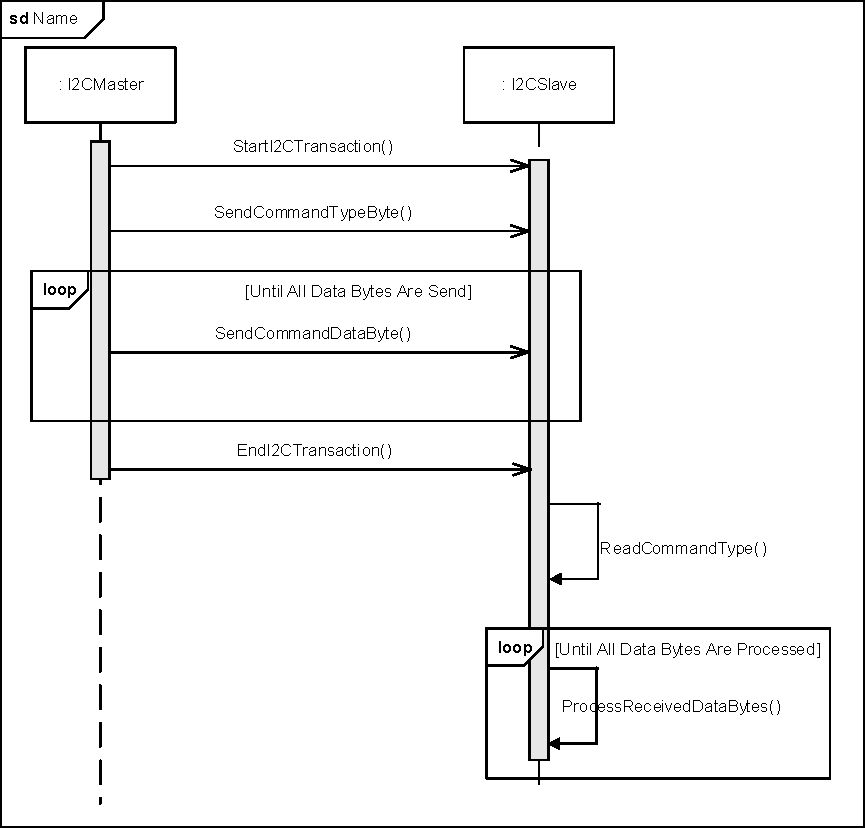
\includegraphics[width=\textwidth] {Systemarkitektur/images/I2CProtocol.pdf}
	\caption{Eksempel af I2C Protokol Forløb}
	\label{fig:I2CProtokolEksempel}
\end{figure}

\noindent På figur \ref{fig:I2CProtokolEksempel} ses, at afsenderen starter en I2C transaktion, hvorefter kommandotypen sendes som den første byte. Efterfølgende sendes \textit{N} antal bytes, afhængig af, hvor meget data den givne kommandotype har brug for at sende. Efter en afsluttet I2C transaktion læser I2C modtageren typen af kommando, hvor den herefter tolker \textit{N} antal modtagne bytes afhængig af den modtagne kommandotype.

\subsubsection{Designvalg}
Den primære idé bag valget af kommandotypemetoden til I2C-kommunikationsprotokollen er først og fremmest at give  mulighed for, at modtageren kan differentiere mellem flere handlinger i systemet. En anden vigtig grund er, at der ved kommandotyper kan associeres et dynamisk antal bytes til hver kommando. Det vil sige, at hvis en modtager får en kommandotype \textit{A}, vil den vide, at der efterfølgende skal læses 5 bytes, hvormiod at en kommandotype \textit{B} ville betyde, at der kun skulle læses 2 bytes.\newline

\noindent En anden fordel ved kommandotypemetoden er, at den er relativt simpel at implementere i kode som vist ved pseudofunktionerne i figur \ref{fig:I2CProtokolEksempel}.

\subsection{Brugergrænseflade}
Ved hjælp af en brugergrænseflade, kan systemtesten styres fra Devkit 8000.
Brugergrænsefladen er opbygget ud fra sekvensdiagrammet på figur \ref{fig:SystemTestSekvensDiagram}, og ud fra dette kunne brugergrænsefladen skitseres som på figur \ref{fig:GUISkitse}.
Grænsefladen mellem Devkit 8000 og PSoC0 er en SPI-bus som ses på figur \ref{afsnit:IBD}, og brugergrænsefladen er koblet til Devkit 8000 ved hjælp af interfacedriveren.
Brugergrænsefladen skal sende startsekvensen til interfacedriveren, hvorefter dette sendes til PSoC0 og videre ud i systemet, som beskrevet i sekvensdiagrammet figur \ref{fig:SystemTestSekvensDiagram}.
Brugergrænsefladen skal aflæse svaret fra systemtesten og printe dette ud i en konsol.

\begin{figure}[H]
	\centering
	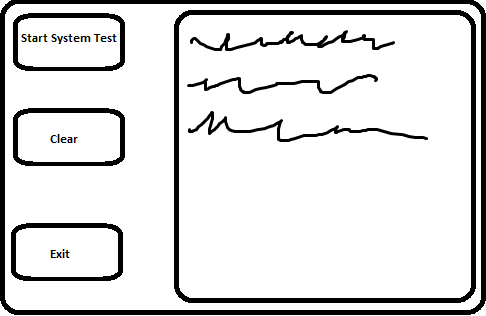
\includegraphics[width=\textwidth] {Systemarkitektur/images/GUISkitse}
	\caption{Skitse af brugergrænseflade}
	\label{fig:GUISkitse}
\end{figure}

\subsubsection{Designvalg}
Brugergrænsefladen er designet ud fra den sekventielle struktur i use case 2, hvilken er beskrevet i afsnit \ref{afsnit:usecasebeskrivelseUC2} og i dokumentationen afsnit 3.5.2-\textit{Use case 2 - Test kommunikationsprotokoller} side 32. Dette er løst ved hjælp af Event-Driven Programming.
Denne model drives ved hjælp af events, som i dette tilfælde aktiveres af brugeren ved knaptryk. Knapperne vil blive tildelt forskellige funktionaliteter, der faciliterer systemtesten.
Et alternativ kunne være trådbaseret design. Kompleksiteten i dette design ville være overvældende i forhold til den ønskede funktionalitet og blev derfor fravalgt.